%package list
\documentclass{article}
\usepackage[top=3cm, bottom=3cm, outer=3cm, inner=3cm]{geometry}
\usepackage{multicol}
\usepackage{graphicx}
\usepackage{url}
%\usepackage{cite}
\usepackage{hyperref}
\usepackage{array}
%\usepackage{multicol}
\newcolumntype{x}[1]{>{\centering\arraybackslash\hspace{0pt}}p{#1}}
\usepackage{natbib}
\usepackage{pdfpages}
\usepackage{multirow}    
\usepackage[normalem]{ulem}
\useunder{\uline}{\ul}{}
\usepackage{svg}
\usepackage{xcolor}
\usepackage{listings}
\lstdefinestyle{ascii-tree}{
    literate={├}{|}1 {─}{--}1 {└}{+}1 
  }

\lstset{basicstyle=\ttfamily,
  showstringspaces=false,
  commentstyle=\color{red},
  keywordstyle=\color{blue}
}
%\usepackage{booktabs}
\usepackage{caption}
\usepackage{subcaption}
\usepackage{float}
\usepackage{array}

\usepackage{enumitem}


\newcolumntype{M}[1]{>{\centering\arraybackslash}m{#1}}
\newcolumntype{N}{@{}m{0pt}@{}}


%%%%%%%%%%%%%%%%%%%%%%%%%%%%%%%%%%%%%%%%%%%%%%%%%%%%%%%%%%%%%%%%%%%%%%%%%%%%
%%%%%%%%%%%%%%%%%%%%%%%%%%%%%%%%%%%%%%%%%%%%%%%%%%%%%%%%%%%%%%%%%%%%%%%%%%%%
\newcommand{\itemEmail}{vmaldonadov@unsa.edu.pe}
\newcommand{\itemStudent}{Victor Gonzalo Maldonado Vilca}
\newcommand{\itemCourse}{Programación Web 2}
\newcommand{\itemCourseCode}{1702122}
\newcommand{\itemSemester}{III}
\newcommand{\itemUniversity}{Universidad Nacional de San Agustín de Arequipa}
\newcommand{\itemFaculty}{Facultad de Ingeniería de Producción y Servicios}
\newcommand{\itemDepartment}{Departamento Académico de Ingeniería de Sistemas e Informática}
\newcommand{\itemSchool}{Escuela Profesional de Ingeniería de Sistemas}
\newcommand{\itemAcademic}{2024 - A}
\newcommand{\itemInput}{Del 29 de mayo de 2024}
\newcommand{\itemOutput}{Al 1 de junio de 2024}
\newcommand{\itemPracticeNumber}{05}
\newcommand{\itemTheme}{Django}
%%%%%%%%%%%%%%%%%%%%%%%%%%%%%%%%%%%%%%%%%%%%%%%%%%%%%%%%%%%%%%%%%%%%%%%%%%%%
%%%%%%%%%%%%%%%%%%%%%%%%%%%%%%%%%%%%%%%%%%%%%%%%%%%%%%%%%%%%%%%%%%%%%%%%%%%%

\usepackage[english,spanish]{babel}
\usepackage[utf8]{inputenc}
\AtBeginDocument{\selectlanguage{spanish}}
\renewcommand{\figurename}{Figura}
\renewcommand{\refname}{Referencias}
\renewcommand{\tablename}{Tabla} %esto no funciona cuando se usa babel
\AtBeginDocument{%
	\renewcommand\tablename{Tabla}
}

\usepackage{fancyhdr}
\pagestyle{fancy}
\fancyhf{}
\setlength{\headheight}{30pt}
\renewcommand{\headrulewidth}{1pt}
\renewcommand{\footrulewidth}{1pt}
\fancyhead[L]{\raisebox{-0.2\height}{
\includegraphics[width=3cm]{img/logo_episunsa.png}}}
\fancyhead[C]{\fontsize{7}{7}\selectfont	\itemUniversity \\ \itemFaculty \\ \itemDepartment \\ \itemSchool \\ \textbf{\itemCourse}}
\fancyhead[R]{\raisebox{-0.2\height}{
\includegraphics[width=1.2cm]{img/logo_abet}}}
\fancyfoot[L]{Victor M.}
\fancyfoot[C]{\itemCourse}
\fancyfoot[R]{Página \thepage}

% para el codigo fuente
\usepackage{listings}
\usepackage{color, colortbl}
\definecolor{dkgreen}{rgb}{0,0.6,0}
\definecolor{gray}{rgb}{0.5,0.5,0.5}
\definecolor{mauve}{rgb}{0.58,0,0.82}
\definecolor{codebackground}{rgb}{0.95, 0.95, 0.92}
\definecolor{tablebackground}{rgb}{0.8, 0, 0}

\lstset{frame=tb,
	language=bash,
	aboveskip=3mm,
	belowskip=3mm,
	showstringspaces=false,
	columns=flexible,
	basicstyle={\small\ttfamily},
	numbers=none,
	numberstyle=\tiny\color{gray},
	keywordstyle=\color{blue},
	commentstyle=\color{dkgreen},
	stringstyle=\color{mauve},
	breaklines=true,
	breakatwhitespace=true,
	tabsize=3,
	backgroundcolor= \color{codebackground},
}

\begin{document}
	
	\vspace*{10px}
	
	\begin{center}	
		\fontsize{17}{17} \textbf{ Informe de Django }
	\end{center}
	\centerline{\textbf{\Large Tema: \itemTheme}}
	%\vspace*{0.5cm}	

	\begin{flushright}
		\begin{tabular}{|M{2.5cm}|N|}
			\hline 
			\rowcolor{tablebackground}
			\color{white} \textbf{Nota}  \\
			\hline 
			     \\[30pt]
			\hline 			
		\end{tabular}
	\end{flushright}	

	\begin{table}[H]
		\begin{tabular}{|x{4.7cm}|x{4.8cm}|x{4.8cm}|}
			\hline 
			\rowcolor{tablebackground}
			\color{white} \textbf{Estudiante} & \color{white}\textbf{Escuela}  & \color{white}\textbf{Asignatura}   \\
			\hline 
			{\itemStudent \par \itemEmail} & \itemSchool & {\itemCourse \par Semestre: \itemSemester \par Código: \itemCourseCode}     \\
			\hline 			
		\end{tabular}
	\end{table}		
	
	\begin{table}[H]
		\begin{tabular}{|x{4.7cm}|x{4.8cm}|x{4.8cm}|}
			\hline 
			\rowcolor{tablebackground}
			\color{white}\textbf{Tarea} & \color{white}\textbf{Tema}  & \color{white}\textbf{Duración}   \\
			\hline 
			\itemPracticeNumber & \itemTheme & 2 horas   \\
			\hline 
		\end{tabular}
	\end{table}
	
	\begin{table}[H]
		\begin{tabular}{|x{4.7cm}|x{4.8cm}|x{4.8cm}|}
			\hline 
			\rowcolor{tablebackground}
			\color{white}\textbf{Semestre académico} & \color{white}\textbf{Fecha de inicio}  & \color{white}\textbf{Fecha de entrega}   \\
			\hline 
			\itemAcademic & \itemInput &  \itemOutput  \\
			\hline 
		\end{tabular}
	\end{table}
%%%%%%%%%%%%%%%%%%%%

  \section{Introducción}
  Django es un framework de desarrollo web en Python que facilita la creación rápida de aplicaciones web seguras y escalables.
  Ofrece un conjunto de herramientas integradas como ORM, administrador de Django y enrutamiento de URLs, lo que simplifica el 
  desarrollo y mejora la seguridad de las aplicaciones web.

%%%%%%%%%%%%%%%%%%%%

  \section{Objetivos}
  \begin{itemize}
    \item Entender y configurar el entorno de trabajo para Django
    \item Crear un primer proyecto en Django
    \item Crear apps e integrarlas al framework
  \end{itemize}

%%%%%%%%%%%%%%%%%%%%
 
	\section{Tarea}
  En esta tarea deberá seguir las diapositivas de DJango01, dentro de un proyecto git local, deberá hacer un commit 
  por cada paso, si desea puede usar branch. La entrega de la tarea consistirá de una captura de pantalla (png o jpg) 
  del siguiente comando:
  \newline
  git log --graph --pretty=oneline --abbrev-commit --all
  \newline
  Cada commit debe ser realizado con un mensaje descriptivo del paso de la diapositiva que estuvo siguiendo.
  \newpage
  La calificación tendrá en cuenta los siguientes aspectos:
  \begin{itemize}
    \item Presentó la tarea 10 puntos
    \item Los mensajes de los commit son claros y descriptivos 10 puntos
    \item Realizó Branch +2 puntos extra
  \end{itemize}
 
%%%%%%%%%%%%%%%%%%%% 
 
  \section{Entregables}
  \begin{itemize}
    \item Informe hecho en Latex
    \item Captura de pantalla (png o jpg) del comando:
    \begin{lstlisting}
    git log --graph --pretty=oneline --abbrev-commit --all
    \end{lstlisting}
    
    \item EXTRA: URL del repositorio en GitHub
  \end{itemize}
  
%%%%%%%%%%%%%%%%%%%%    
		
	\section{Equipos, materiales y temas utilizados}
  \begin{itemize}
    \item Python
    \item Pip
    \item Django
    \item Entornos virtuales en python
    \item Proyectos de Django
    \item Aplicaciones en Django
    \item Modelos, Vistas, Templates y Formularios en Django
  \end{itemize}
 
%%%%%%%%%%%%%%%%%%%%

  \section{Captura de pantalla (png o jpg)}
  \begin{itemize}
    \item \textbf{Comando usado:}
    \begin{lstlisting}
    git log --graph --pretty=oneline --abbrev-commit --all
    \end{lstlisting}
    \newpage
    \item \textbf{Captura:}
    \begin{figure}[H]
      \centering
      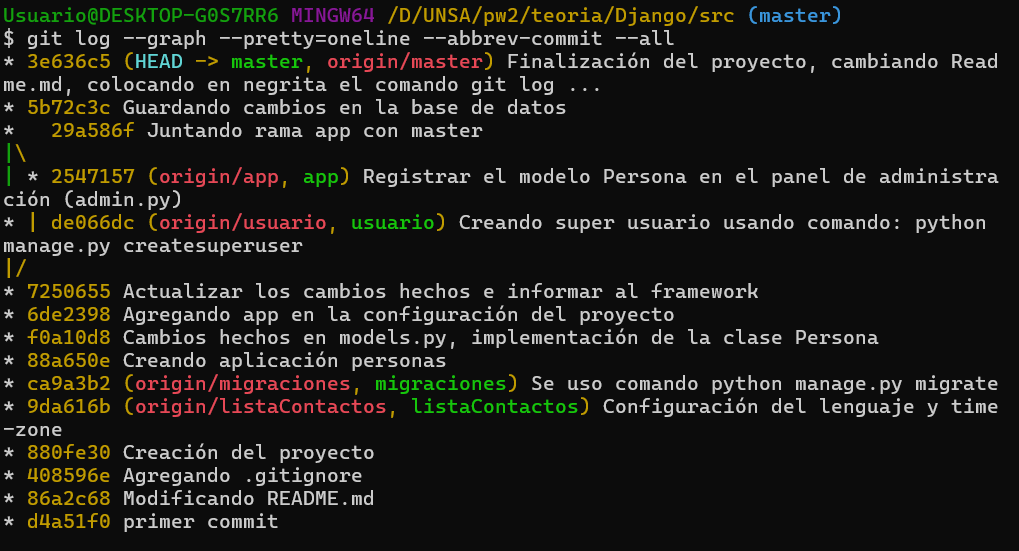
\includegraphics[width=1\textwidth, keepaspectratio]{img/captura.png}
      \caption{Captura del comando git}
    \end{figure} 
  \end{itemize}
  
%%%%%%%%%%%%%%%%%%%%

	\section{URL de Repositorio Github}
  \begin{itemize}
    \item URL: Repositorio GitHub
    \item \url{https://github.com/Victor-Gonzalo-Maldonado-Vilca/Django.git}
  \end{itemize}

%%%%%%%%%%%%%%%%%%%%

  \section{Metodología}
  
%%%%%%%%%%%%
  
  \subsection{Creación del entorno de Trabajo}
  
%%%%%%

  \subsubsection{Carpeta de trabajo}
  \begin{lstlisting}[language=, caption={Creación del Directorio}]
  mkdir Django && cd Django
  \end{lstlisting}
  
%%%%%%

  \subsubsection{Creación del Entorno Virtual}
  \begin{lstlisting}[language=, caption={Creación Entorno virtual}]
  virtualenv -p python3 .
  \end{lstlisting}
  \newpage
  
%%%%%%%

  \subsubsection{Activar entorno Virtual}
  \begin{lstlisting}[language=, caption={Activar Entorno Virtual}]
  Scripts/activate
  \end{lstlisting}
  
%%%%%%

  \subsubsection{Instalar Django en el entorno Virtual}
  \begin{lstlisting}[language=, caption={Instalar Django}]
  pip install Django
  \end{lstlisting}
  
%%%%%%

  \subsubsection{Creación carpeta del proyecto}
  \begin{lstlisting}[language=, caption={Carpeta src}]
  mkdir src && cd src
  \end{lstlisting}
  
%%%%%%

  \subsubsection{Inicializar git}
  \begin{lstlisting}[language=, caption={Inicializar git}]
  git init
  \end{lstlisting}
  
%%%%%%

  \subsubsection{Crear .gitignore}
  Seguimos el siguiente Repositorio \url{https://github.com/django/django/blob/main/.gitignore}
  
%%%%%%%%%%%%
  
  \subsection{Creacion del proyecto y apps}
  
%%%%%%

  \subsubsection{Crear Proyecto}
  \begin{lstlisting}[language=, caption={Crear proyecto}]
  django-admin startproject listaContactos
  \end{lstlisting}
  
%%%%%%

  \subsubsection{Crear App}
  \begin{lstlisting}[language=, caption={Crear App}]
  python manage.py startapp personas
  \end{lstlisting}
  \newpage

%%%%%%%%%%%%%%%%%%%%

  \section{Desarrollo del trabajo}
 
%%%%%%%%%%%%
 
  \subsection{Configuramos el proyecto en settings.py}
  
%%%%%%

  \subsubsection{Cambiamos el idioma y zona del tiempo}
  \begin{figure}[H]
    \centering
    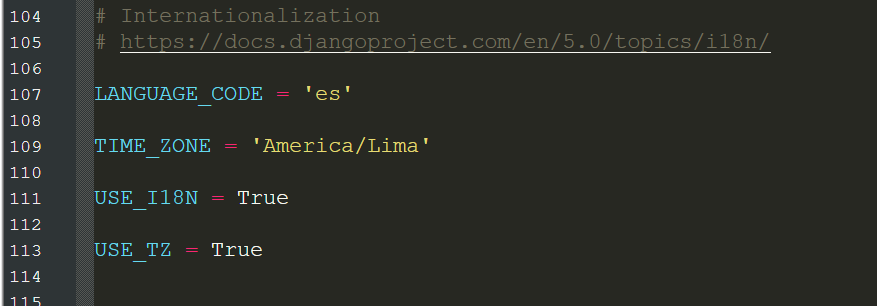
\includegraphics[width=1\textwidth, keepaspectratio]{img/lenguaje.png}
    \caption{Configuración a nuestra región}
  \end{figure}

%%%%%%

  \subsubsection{Migraciones}
  \textit{Uso del comando: python manage.py migrate}
  \begin{figure}[H]
    \centering
    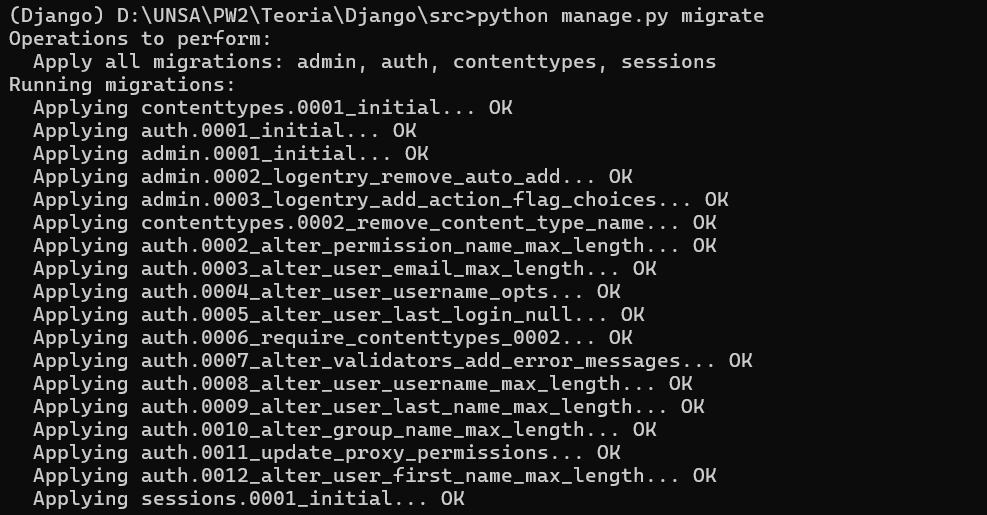
\includegraphics[width=1\textwidth, keepaspectratio]{img/migraciones.png}
    \caption{migraciones}
  \end{figure}
  \newpage
  
%%%%%%

  \subsubsection{Agregamos la aplicación en el archivo settings.py}
  \begin{figure}[H]
    \centering
    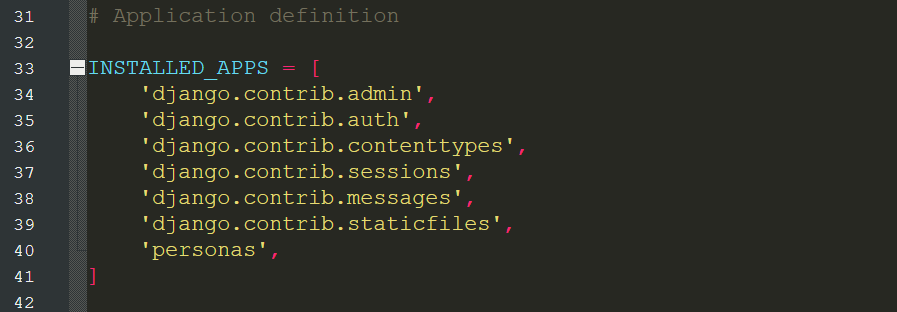
\includegraphics[width=1\textwidth, keepaspectratio]{img/app.png}
    \caption{Agregar App}
  \end{figure}
  
%%%%%%%%%%%%

  \subsection{Definir Modelos en models.py en la App personas}
  
%%%%%%

  \subsubsection{Modelo Persona}
  \begin{itemize}
    \item \textbf{Modelo Persona:}
    \begin{figure}[H]
      \centering
      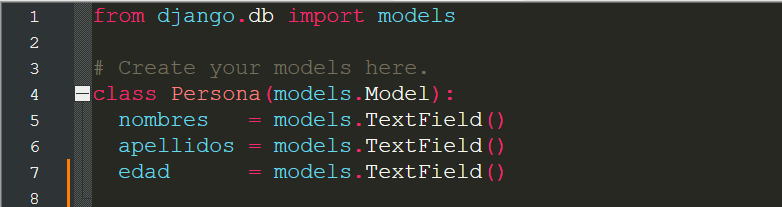
\includegraphics[width=1\textwidth, keepaspectratio]{img/modelo.png}
      \caption{Modelo Persona}
    \end{figure}  
  \end{itemize}
  
%%%%%%%%%%%%

  \subsection{Actualizar los cambios hechos e informar al framework}
  
%%%%%%
  
  \subsubsection{Informar al Framework sobre los cambios}
  \begin{lstlisting}[language=, caption={Comando}]
  python manage.py makemigrations
  \end{lstlisting}
  \begin{figure}[H]
    \centering
    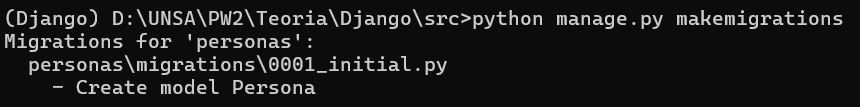
\includegraphics[width=1\textwidth, keepaspectratio]{img/informar.png}
    \caption{Informar al Framework}
  \end{figure}
  \newpage
  
%%%%%%
  
  \subsubsection{Actualizar los cambios hechos}
  \begin{lstlisting}[language=, caption={Comando}]
  python manage.py migrate
  \end{lstlisting}
  \begin{figure}[H]
    \centering
    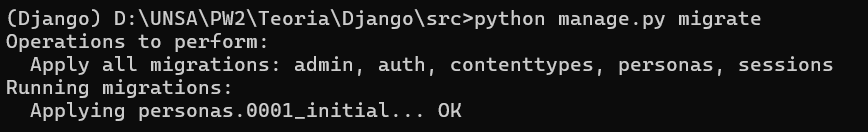
\includegraphics[width=1\textwidth, keepaspectratio]{img/actualizar.png}
    \caption{Actualizar}
  \end{figure}
  
%%%%%%%%%%%%

  \subsection{Creando nuevo usuario}
  \textit{Crear un nuevo usuario con su contraseña y con permisos de administrador}
  \begin{itemize}
    \item \textbf{Uso del comando: }
    \begin{lstlisting}
    python manage.py createsuperuser
    \end{lstlisting}
    \begin{figure}[H]
      \centering
      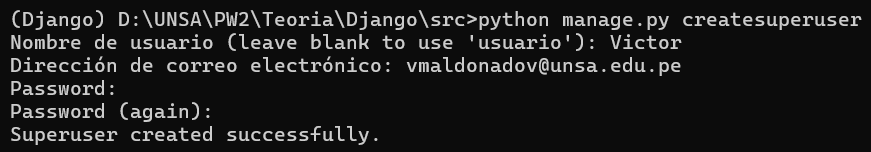
\includegraphics[width=1\textwidth, keepaspectratio]{img/nuevoUsuario.png}
      \caption{Crear Usuario}
    \end{figure}
    \item \textbf{Capturas: }
    \begin{figure}[H]
      \centering
      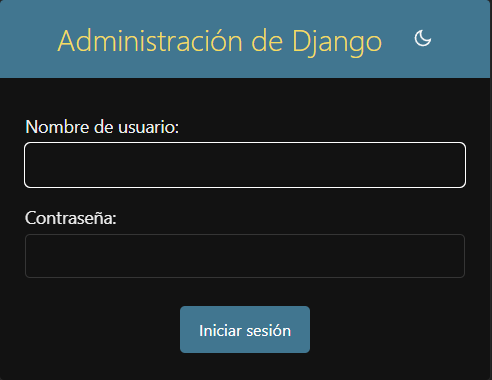
\includegraphics[width=0.5\textwidth, keepaspectratio]{img/admin.png}
      \caption{Captura 1}
    \end{figure}
    \newpage
    \begin{figure}[H]
      \centering
      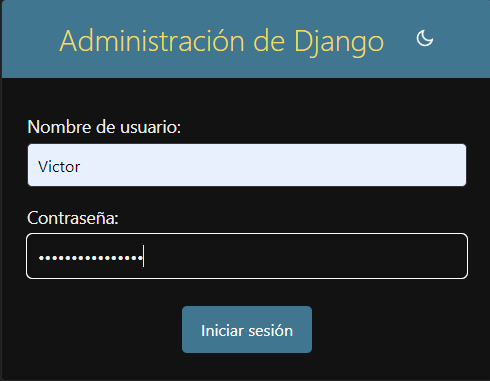
\includegraphics[width=0.5\textwidth, keepaspectratio]{img/admin1.png}
      \caption{Captura 2}
    \end{figure}
    \begin{figure}[H]
      \centering
      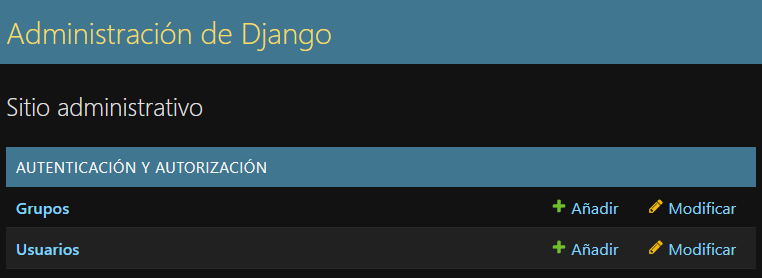
\includegraphics[width=1\textwidth, keepaspectratio]{img/admin2.png}
      \caption{Captura 3}
    \end{figure}
  \end{itemize}
  
%%%%%%%%%%%%

  \subsection{Registro de Modelos en el Administrador (admin.py)}
  \begin{figure}[H]
    \centering
    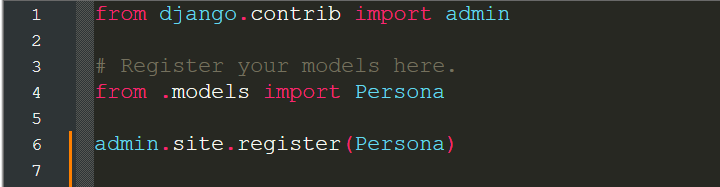
\includegraphics[width=1\textwidth, keepaspectratio]{img/administrador.png}
    \caption{admin.py}
  \end{figure}
  \begin{figure}[H]
    \centering
    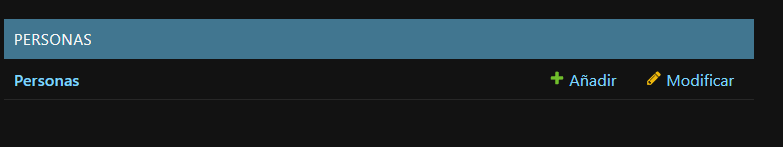
\includegraphics[width=1\textwidth, keepaspectratio]{img/server.png}
    \caption{En el Servidor}
  \end{figure}
  
%%%%%%%%%%%%

  \subsection{Crear nuevo objeto de Persona}
  \begin{itemize}
    \item \textbf{Uso del comando:}
    \begin{lstlisting}
    python manage.py shell
    \end{lstlisting}
    \begin{figure}[H]
      \centering
      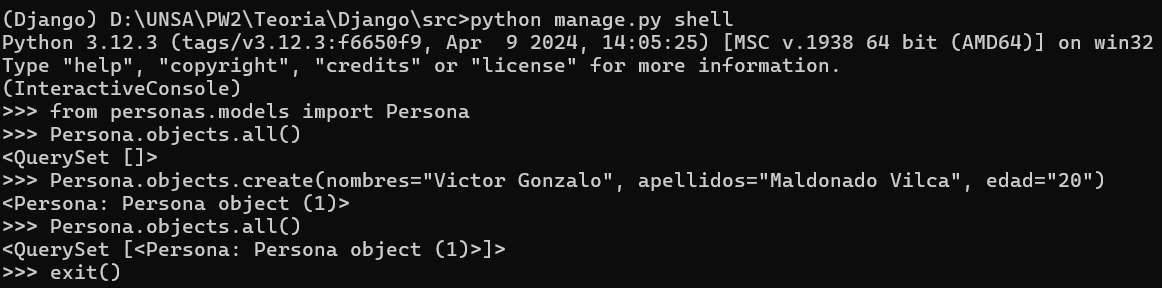
\includegraphics[width=1\textwidth, keepaspectratio]{img/shell.png}
      \caption{Shell}
    \end{figure}
    \begin{figure}[H]
      \centering
      \includegraphics[width=0.8\textwidth, keepaspectratio]{img/Server1.png}
      \caption{En el Servidor}
    \end{figure}
  \end{itemize}
  
%%%%%%%%%%%%

  \subsection{Iniciar el servidor de desarrollo}
  Recordemos que para iniciar el servidor se usa el comando:
  \begin{lstlisting}
  python manage.py runserver
  \end{lstlisting}
  \begin{figure}[H]
    \centering
    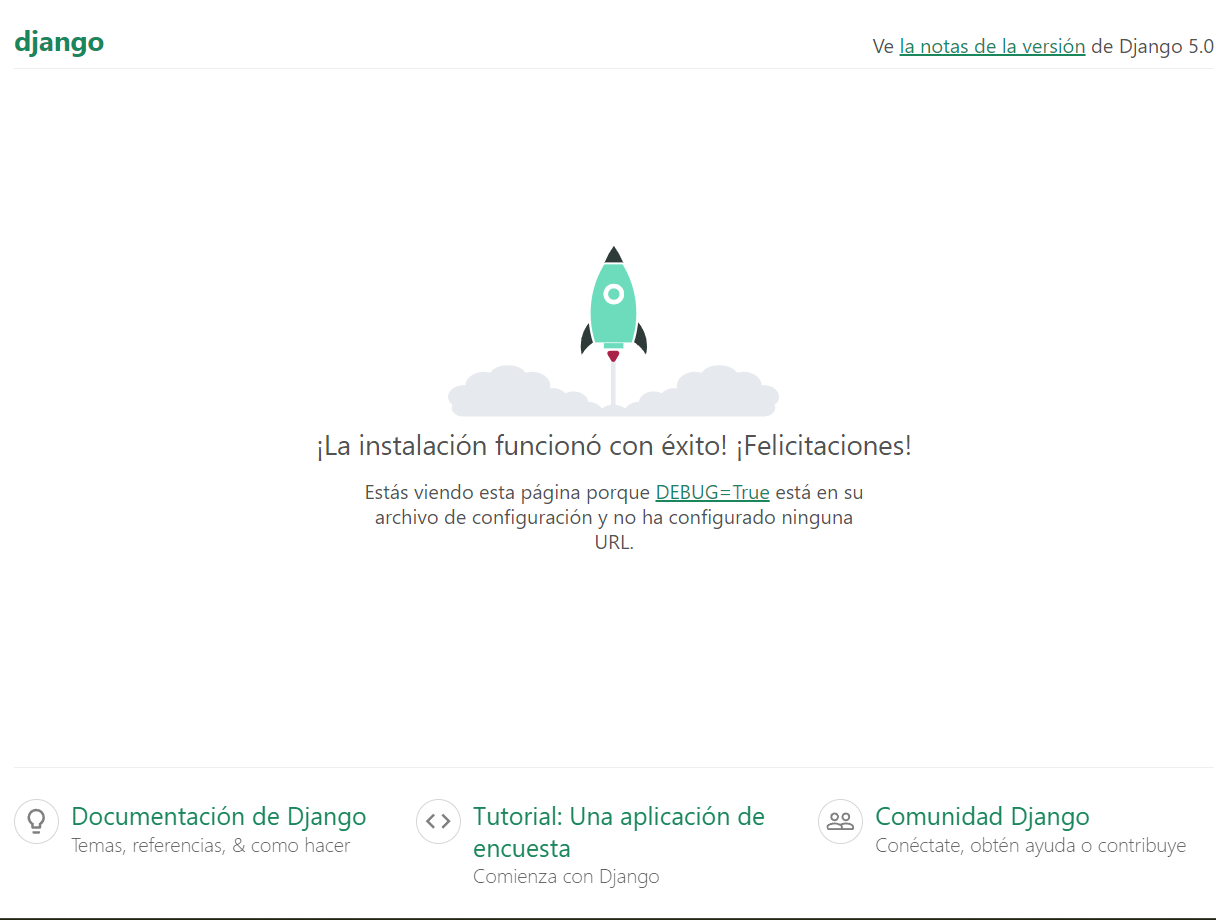
\includegraphics[width=1\textwidth, keepaspectratio]{img/ejecutar.png}
    \caption{Servidor}
  \end{figure}
  \newpage
  Ahora colocando http://127.0.0.1:8000/admin/ ya registrandonos con las credenciales del usuario
  \begin{figure}[H]
    \centering
    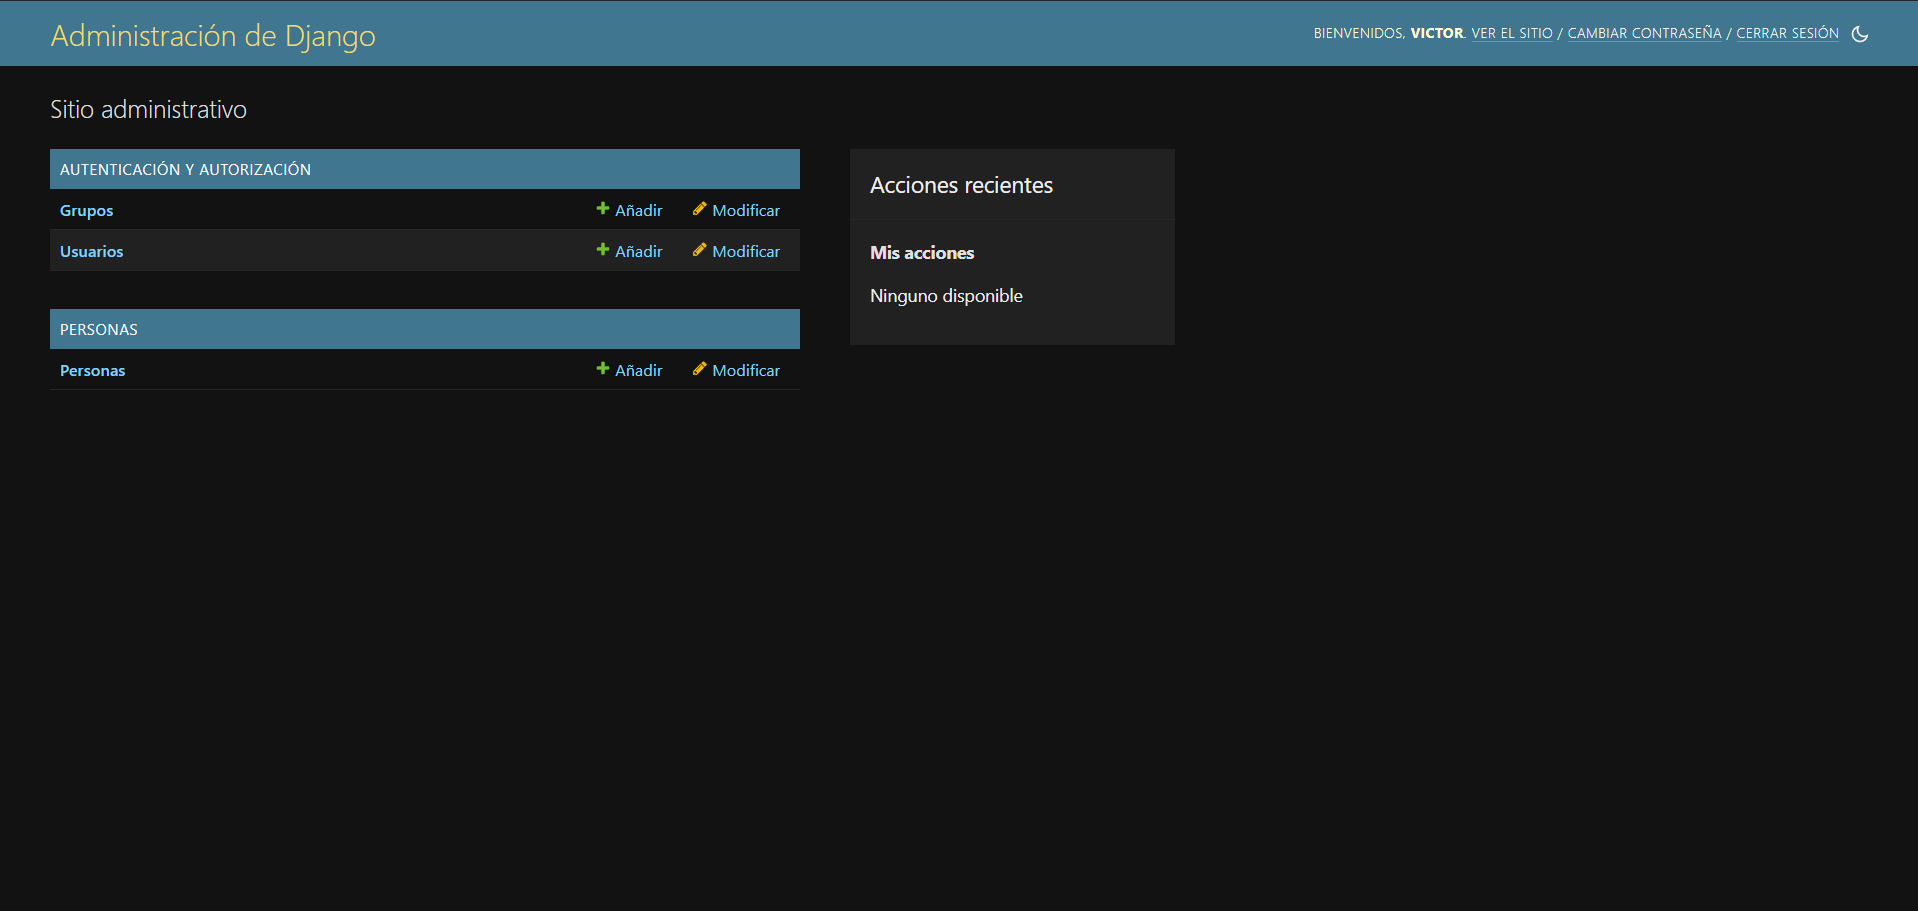
\includegraphics[width=1\textwidth, keepaspectratio]{img/ejecutar1.png}
    \caption{Servidor}
  \end{figure}
    
%%%%%%%%%%%%
	
  \subsection{Uso de GitHub}
  
%%%%%%

	\subsubsection{Usuario de GitHub}
  \begin{figure}[H]
    \centering
    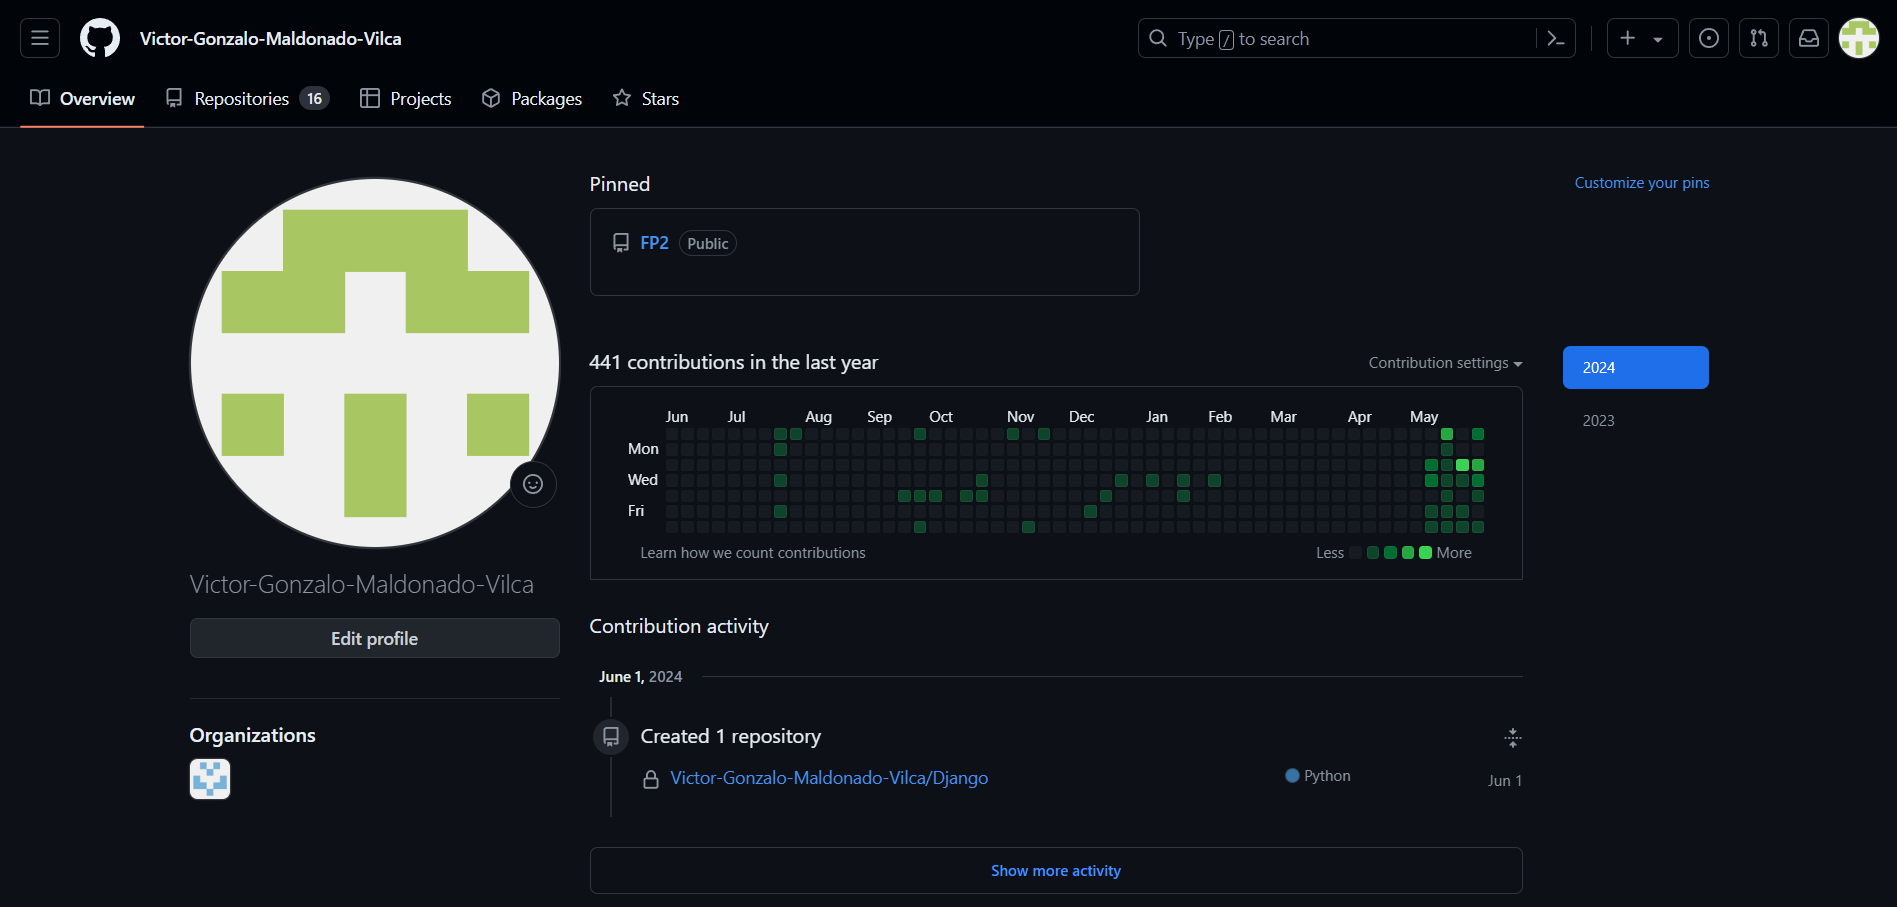
\includegraphics[width=1\textwidth, keepaspectratio]{img/usuario.png}
    \caption{Usuario}
  \end{figure}
  \newpage
  
%%%%%%

  \subsubsection{Creación de un Nuevo Repositorio}
  \begin{figure}[H]
    \centering
    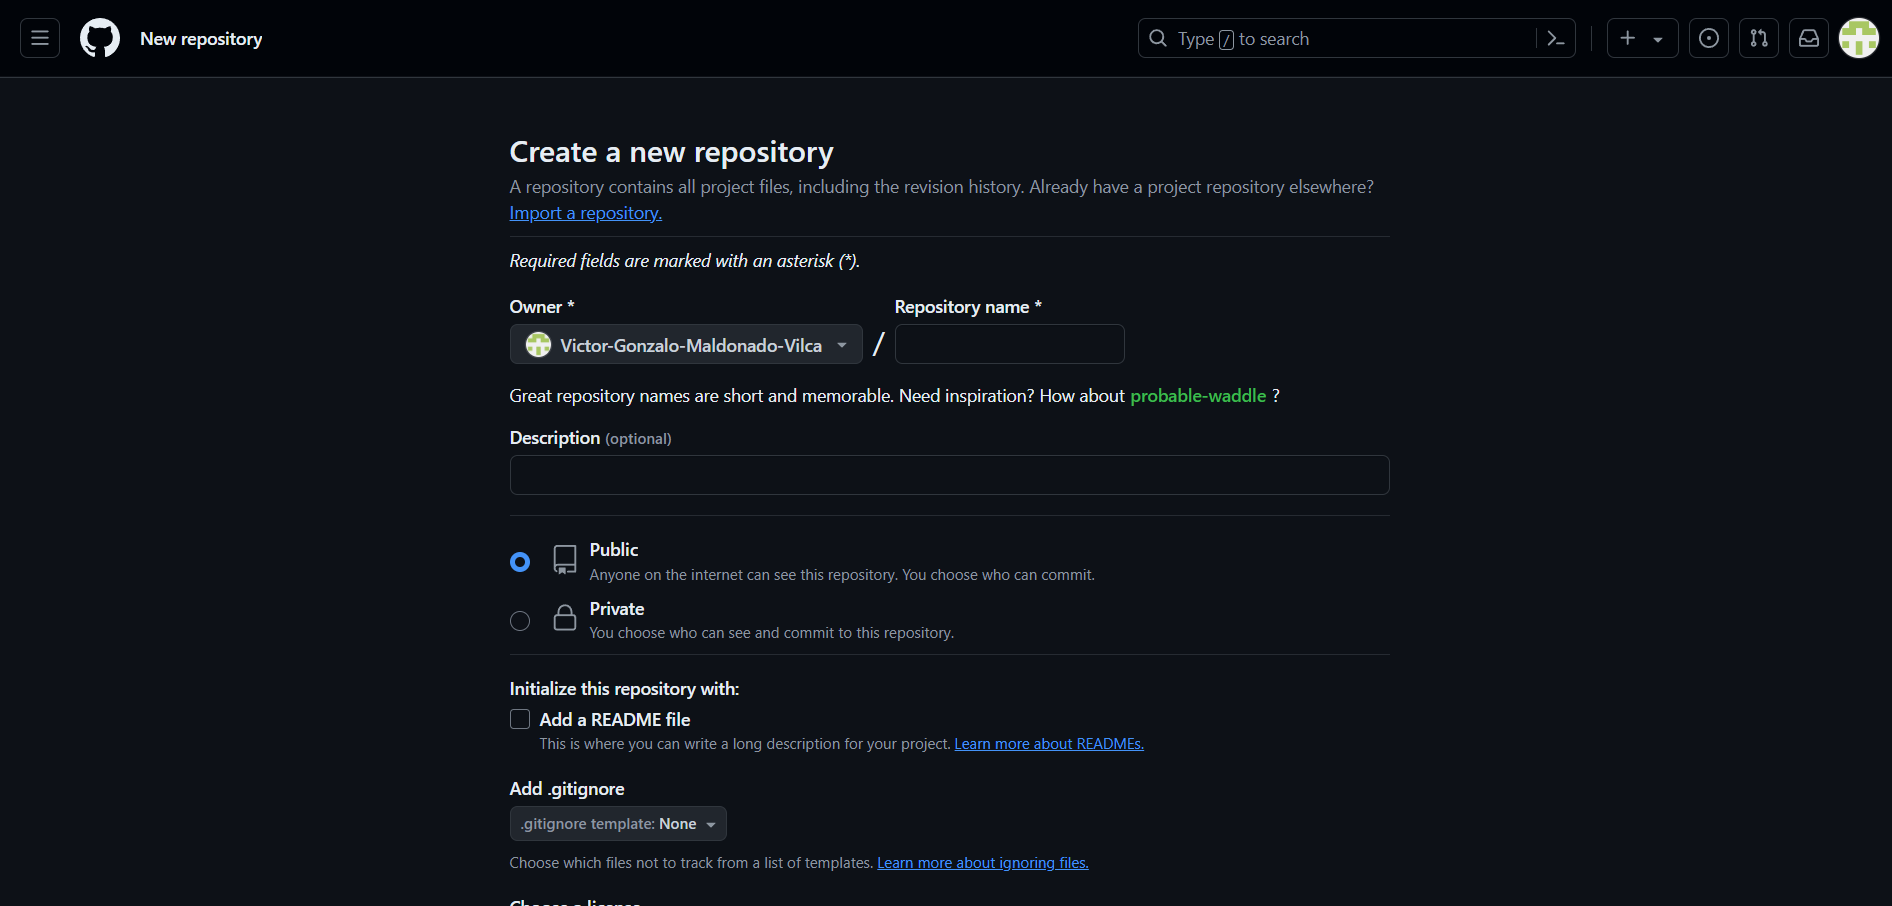
\includegraphics[width=1\textwidth, keepaspectratio]{img/crear.png}
    \caption{Crear Repositorio}
  \end{figure}
  
%%%%%%
	
  \subsubsection{Comandos de Configuración}
  \begin{lstlisting}[language=, caption={Comando Iniciales}]
  echo "# Auxiliar" >> README.md
  git init
  git add README.md
  git commit -m "primer commit"
  git branch -M master
  git remote add origin https://github.com/Victor-Gonzalo-Maldonado-Vilca/Django.git
  git push -u origin master
  \end{lstlisting}
  \newpage
  
%%%%%% 
  
  \subsubsection{Implementación de Readme.md}
  \begin{figure}[H]
    \centering
    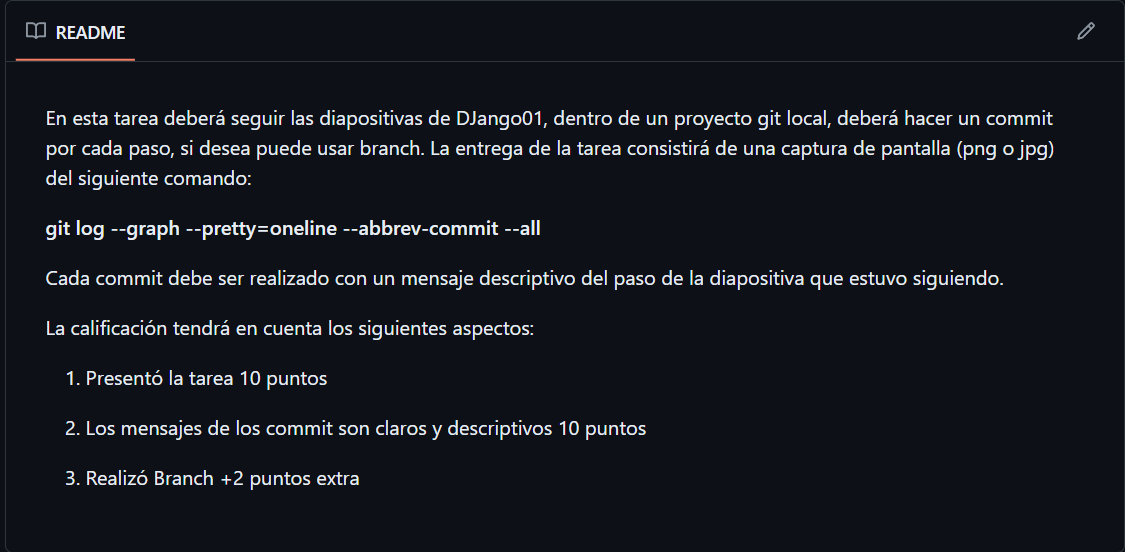
\includegraphics[width=1\textwidth, keepaspectratio]{img/readme.png}
    \caption{README.md}
  \end{figure}
  
%%%%%%

	\subsubsection{Registro de cambios en mi código}
  \begin{figure}[H]
    \centering
    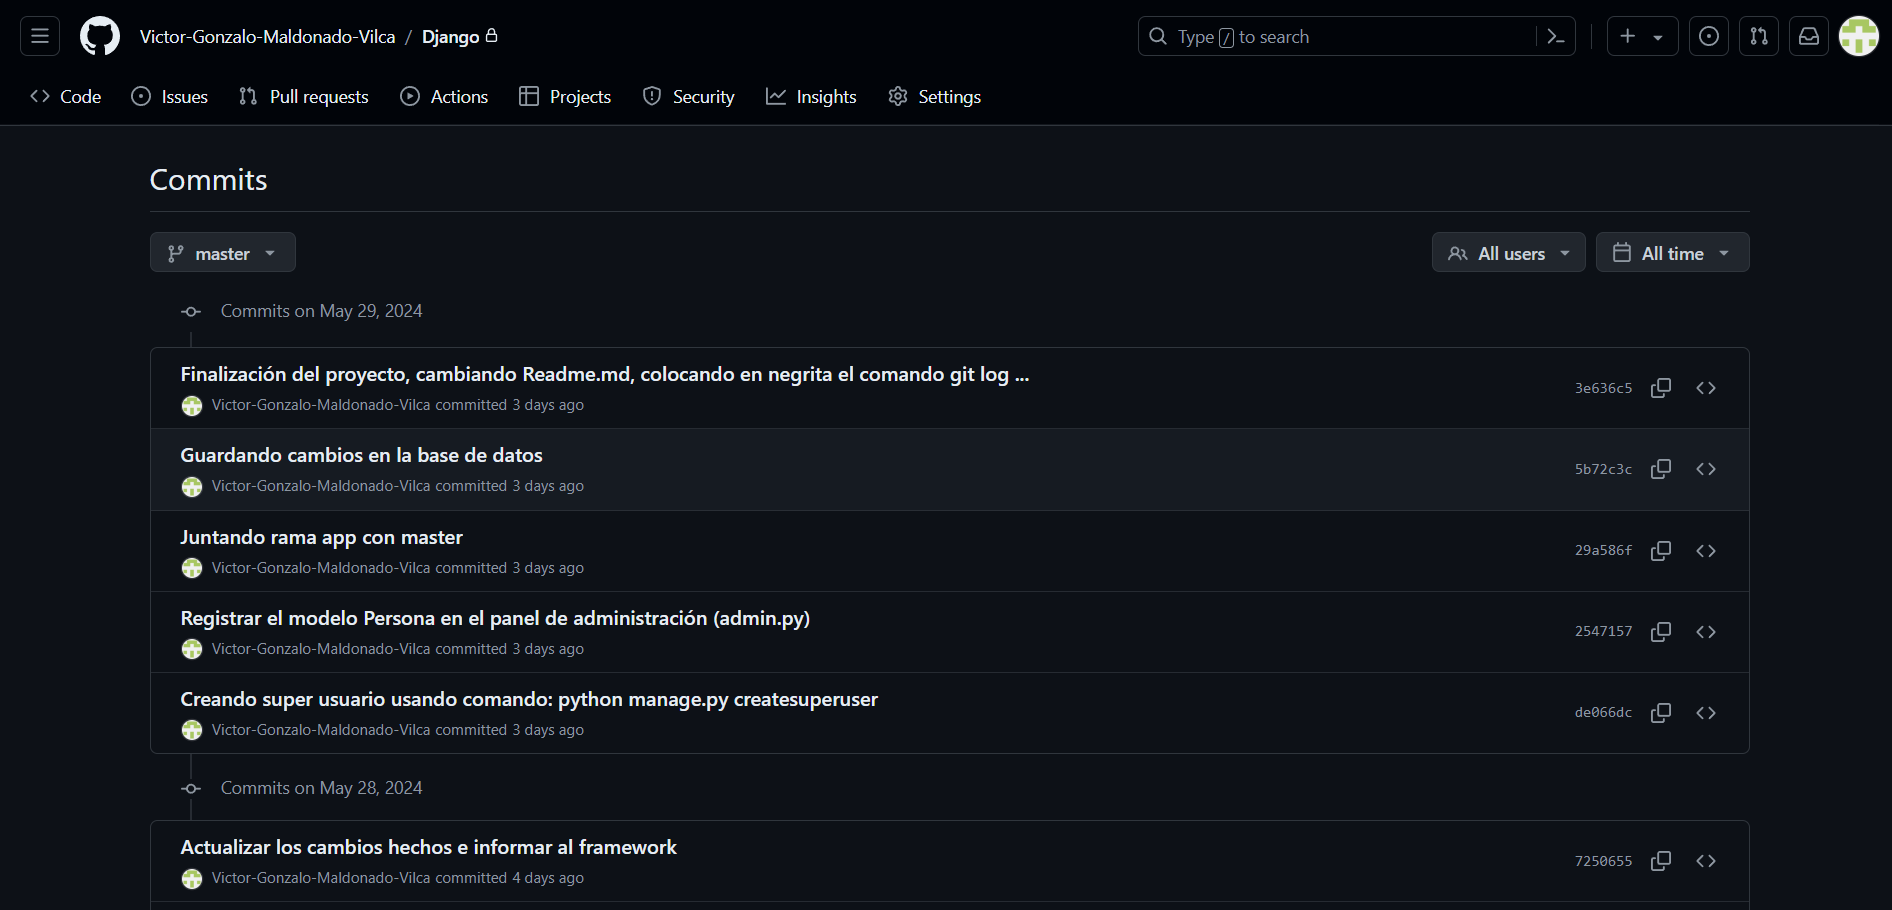
\includegraphics[width=1\textwidth, keepaspectratio]{img/commits.png}
    \caption{Commits}
  \end{figure}
  \newpage
	
%%%%%%

	\subsubsection{Repositorio}
  \begin{figure}[H]
    \centering
    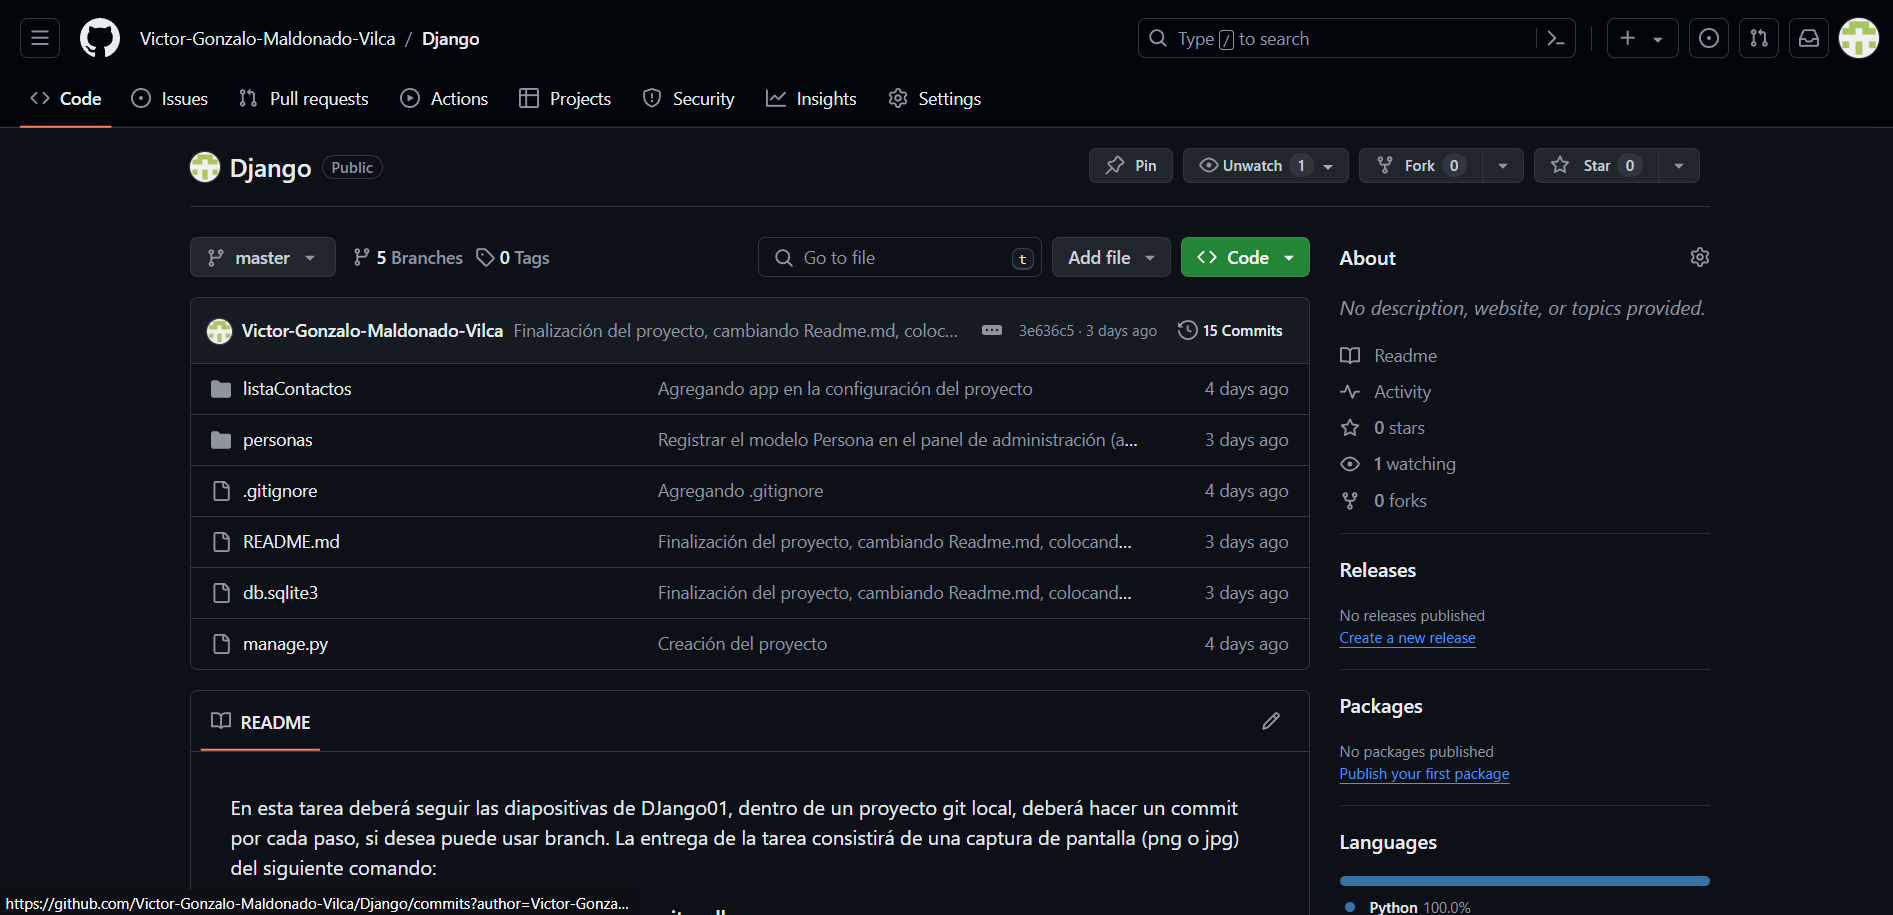
\includegraphics[width=1\textwidth, keepaspectratio]{img/repo.png}
    \caption{Repositorio}
  \end{figure}
  
%%%%%%

	\subsubsection{Uso de Ramas}
  \begin{figure}[H]
    \centering
    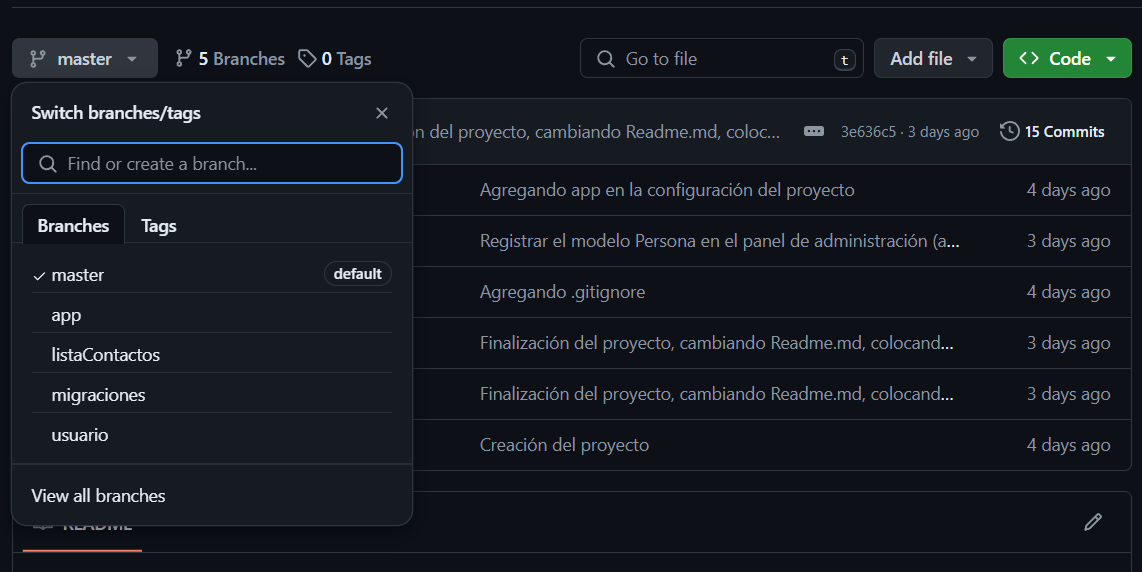
\includegraphics[width=1\textwidth, keepaspectratio]{img/ramas.png}
    \caption{Uso de Ramas}
  \end{figure}
  \newpage

%%%%%%

	\subsubsection{Proyecto compartido con el profesor de github}
  \begin{figure}[H]
    \centering
    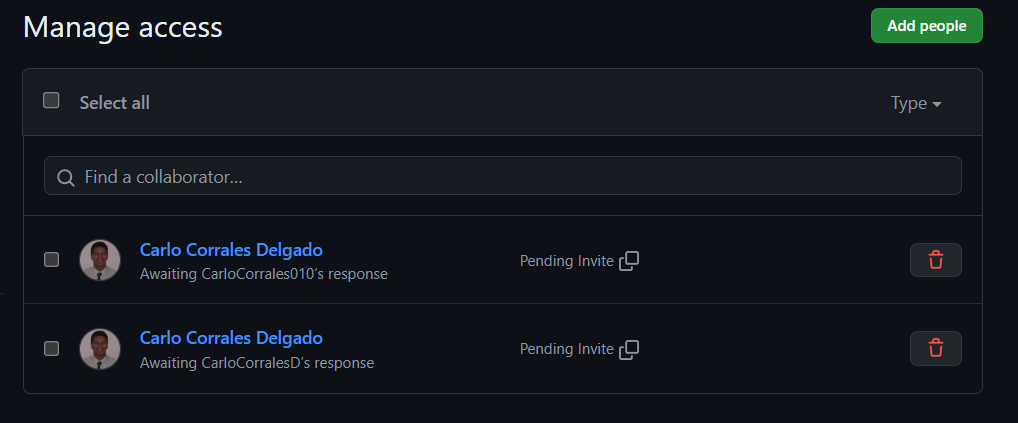
\includegraphics[width=1\textwidth, keepaspectratio]{img/compartir.png}
    \caption{Compartir con el Docente}
  \end{figure}
  
%%%%%%%%%%%%%%%%%%%%

  \section{Recomensaciones}
  \begin{itemize}
    \item Seguir las mejores prácticas de desarrollo de Django, como la separación de la lógica de negocios en vistas y 
    la creación de plantillas reutilizables.
    \item Realizar pruebas unitarias y de integración para garantizar la calidad del código, y asegúrate de implementar 
    medidas de seguridad en tu aplicación.
  \end{itemize}
  
%%%%%%%%%%%%%%%%%%%%

  \section{Conclusiones}
  \begin{itemize}
    \item Django es un framework web potente y versátil que permite desarrollar aplicaciones web de manera rápida y eficiente.
    \item La arquitectura MVC (Modelo-Vista-Controlador) de Django ayuda a organizar el código de manera estructurada y modular, 
    lo que facilita la mantenibilidad y escalabilidad de las aplicaciones.
    \item Con un buen entendimiento de Django y siguiendo las mejores prácticas de desarrollo, se pueden crear aplicaciones web 
    robustas y de alto rendimiento.
  \end{itemize}

%%%%%%%%%%%%%%%%%%%%
	\newpage
	\subsection{\textcolor{red}{Rúbrica para el contenido del Informe y demostración}}
	\begin{itemize}			
		\item El alumno debe marcar o dejar en blanco en celdas de la columna \textbf{Checklist} si cumplio con el ítem correspondiente.
		\item Si un alumno supera la fecha de entrega,  su calificación será sobre la nota mínima aprobada, siempre y cuando cumpla con todos lo items.
		\item El alumno debe autocalificarse en la columna \textbf{Estudiante} de acuerdo a la siguiente tabla:
	
		\begin{table}[ht]
			\caption{Niveles de desempeño}
			\begin{center}
			\begin{tabular}{ccccc}
    			\hline
    			 & \multicolumn{4}{c}{Nivel}\\
    			\cline{1-5}
    			\textbf{Puntos} & Insatisfactorio 25\%& En Proceso 50\% & Satisfactorio 75\% & Sobresaliente 100\%\\
    			\textbf{2.0}&0.5&1.0&1.5&2.0\\
    			\textbf{4.0}&1.0&2.0&3.0&4.0\\
    		\hline
			\end{tabular}
		\end{center}
	\end{table}	
	

	\end{itemize}

 
	
	\begin{table}[H]
		\caption{Rúbrica para contenido del Informe y demostración}
		\setlength{\tabcolsep}{0.5em} % for the horizontal padding
		{\renewcommand{\arraystretch}{1.5}% for the vertical padding
		%\begin{center}
		\begin{tabular}{|p{2.7cm}|p{7cm}|x{1.3cm}|p{1.2cm}|p{1.5cm}|p{1.1cm}|}
			\hline
    		\multicolumn{2}{|c|}{Contenido y demostración} & Puntos & Checklist & Estudiante & Profesor\\
			\hline
			\textbf{1. GitHub} & Hay enlace URL activo del directorio para el  laboratorio hacia su repositorio GitHub con código fuente terminado y fácil de revisar. &2 &X &2 & \\ 
			\hline
			\textbf{2. Commits} &  Hay capturas de pantalla de los commits más importantes con sus explicaciones detalladas. (El profesor puede preguntar para refrendar calificación). &4 &X &4 & \\ 
			\hline 
			\textbf{3. Código fuente} &  Hay porciones de código fuente importantes con numeración y explicaciones detalladas de sus funciones. &2 &X &2 & \\ 
			\hline 
			\textbf{4. Ejecución} & Se incluyen ejecuciones/pruebas del código fuente  explicadas gradualmente. &2 &X &2 & \\ 
			\hline			
			\textbf{5. Pregunta} & Se responde con completitud a la pregunta formulada en la tarea.  (El profesor puede preguntar para refrendar calificación).  &2 &X &2 & \\ 
			\hline	
			\textbf{6. Fechas} & Las fechas de modificación del código fuente estan dentro de los plazos de fecha de entrega establecidos. &2 &X &2 & \\ 
			\hline 
			\textbf{7. Ortografía} & El documento no muestra errores ortográficos. &2 &X &2 & \\ 
			\hline 
			\textbf{8. Madurez} & El Informe muestra de manera general una evolución de la madurez del código fuente,  explicaciones puntuales pero precisas y un acabado impecable.   (El profesor puede preguntar para refrendar calificación).  &4 &X &4 & \\ 
			\hline
			\multicolumn{2}{|c|}{\textbf{Total}} &20 & &20 & \\ 
			\hline
		\end{tabular}
		%\end{center}
		%\label{tab:multicol}
		}
	\end{table}


%%%%%%%%%%%%%%%%%%%%%%%%%%%%%%%%%%%%%%%%%%%%%%%%%%%%%%%%%%%%%%%%%%%
	
  \newpage
  \section{Referencias}
  \begin{itemize}
    \item \url{https://docs.djangoproject.com/en/5.0/}
    \item \url{https://docs.github.com/es}
    \item \url{https://git-scm.com/doc}
  \end{itemize}

%%%%%%%%%%%%%%%%%%%% 
%\clearpage
%\bibliographystyle{apalike}
%\bibliographystyle{IEEEtranN}
%\bibliography{bibliography}
			
\end{document}
